\documentclass[12pt,colorful,boxey]{tufte-style-thesis}

\usepackage{amsmath,amsthm,amsfonts,amssymb,amscd,latexsym}         % ..if you need lots of math symbols
\usepackage{bm}
\usepackage{physics}
\usepackage{mathptmx}
\usepackage{mathtools}
\usepackage{cancel}
\usepackage{centernot} 		% Notacion matematica
\usepackage{empheq}			% Recuadros para ecuaciones
\usepackage[most]{tcolorbox}
\usepackage{comment}
\usepackage{ragged2e}
\usepackage{siunitx}
\usepackage{svg}

\usepackage{algorithm2e}

\bibliographystyle{unsrtnat}

% Insight of mechanical response of hydrogels via patchy particle methodology
% INFO : used in the titlepage, copyright and stuff.
\author{Francisco Javier Vazquez Tavares}
\title{Exploration of mechanical responses of Hydrogels via numerical simulation.}
%\subtitle{This is the subtitle}
\university{Instituto Teconologico de Estudios Superiores de Monterrey}
\person{Supervisor}{Antonio Ortiz Ambriz}{~}
\person{Cosupervisor}{Claudia Elena Ferreiro Crodova}{~}
\person{Jury members}{jury 1}{~}
\person{}{jury 2}{~}
\person{}{jury 3}{~}

%\logo{example-image-a}
%\logo{example-image-b}
%\logo{example-image-c}
\shoutouts{For \ldots}


\begin{document}

\maketitle

\justifying

\chapter*{Abstract}
This thesis explores the theoretical framework necessary for analysing computational simulations of the mechanical response of a network under shear deformation.
This network is modelled on a hydrophilic polymeric network based on a PNIPAM microgel protocol.
The protocol has been implemented in LAMMPS to take advantage of the parallelisation of the velocity Verlet algorithm and Langevin dynamics.
We found that\ldots


\chapter*{Acknowledgements}
\ldots 
Thanks to Tec and SECHIT for the economical support.
\ldots

\tableofcontents
\listoffigures
\listoftables
%\listoflistings


\mainmatter

% Chapters

%======================================================================
\chapter{Introduction}\label{ch1:Intro}

\markright{Introduction}
%======================================================================

\paragraph{Curiosity/phenomenology} Paragraph that will tell the reader that hydrogels are cool.

\paragraph{Applications/Market size of the applications sectors} If the previous paragraph does not convince the reader, well my last hope is that money does.

Besides, because of such a wide variety of response triggers, hydrogels can serve as sensors or actuators or can be utilized in controlled drug delivery systems, biosensors, tissue engineering scaffolds, and others [20], because of their biomimetic properties and multi functionalities [21]\citep{bustamantetorresHydrogelsClassificationAccording2021}.

In particular, biomedical applications are very popular and include cell culture [5], wound dressing and healing [2,6], drug delivery [2,7,8], tissue engineering scaffolds [9], bone repair [10], and cartilage regeneration [11]\citep{picchioniHydrogelsBasedDynamic2018}. 
 

\paragraph{Description of the Thesis} What the reader will find in each chapter and section.

\paragraph{Why computers and not rheometers?} Explain how in silico experiments can help to understand the relation between the network and the mechanical response.

\section{State of the art: Hydrogels}\label{ch1:StateArt}

\begin{itemize}
    \item Characteristics
    \item Descriptions 
    \item Synthesis techniques
    \item Cross-linking (Bond breaking)
\end{itemize}

\paragraph{General description of a hydrogel}
A hydrogel is commonly describe as a material composed by a network of polymers chains that exhibits the abilitiy to swell and retain a significant fraction of water within its structure, but will not dissolve in water\citep{ahmedHydrogelPreparationCharacterization2015a,ahmedHydrogelsMicrogelsDriving2025,priyaComprehensiveReviewHydrogel2024,bustamantetorresHydrogelsClassificationAccording2021}.\footnote{the main difference with the microgels, is the size. Hydrogel is bulk, and microgelgel is particle.}
The water absorption capacity, network stability of hydrogels, and the conformation of the network with polymer chains are attributable to crosslinking mechanisms\citep{priyaComprehensiveReviewHydrogel2024,ahmedHydrogelPreparationCharacterization2015a}.
Meanwhile, the polymer chains are predominantly composed with hydrophilic functional groups and can be modified to suit a variety of applications\citep{ahmedHydrogelPreparationCharacterization2015a,priyaComprehensiveReviewHydrogel2024,bustamantetorresHydrogelsClassificationAccording2021}.

% Hydrophilic polymers might be considered as those polymers that contain polar functional groups such as hydroxyl (-OH), carboxyl (-COOH), and amino (-NH2) groups that make them soluble or swelled by water.

While the analysis of the impact of functional groups is important, the present project prioritizes the examination of mechanisms that are more pertinent to the mechanical response. 
The crosslinking mechanisms\footnote{The hydrogels are prepared using different methods like chemical cross-linking of monomers, physical cross-linking using temperature or pH changes, and blending of natural or synthetic polymers.}, in particular, are of particular interest, as they are responsible for resisting dissolution. 
This suggests that crosslinking mechanisms enable the network to undergo modification by external stimuli.

The subsequent sections will present the essential information to facilitate a comprehensive understanding of the crosslinking mechanisms, their relationship to the mechanical response, the reported mechanical response of hydrogels, and the correlation between rheology experiments and stress curves.


\section{Polymeric Structure}

\paragraph{Overview} The chemical and topological structure of polymer networks are interconnected, influencing their overall characteristics.
The chemical structure is defined by the chemical composition of the network components. 
Tuning this structure effectively enables the incorporation of functions to polymer networks.
In contrast, polymer network topology refers to the configuration of junctions and strands within a polymer network.
Given that many properties of polymer networks (e.g., elasticity, porosity, and swellability) have topological origins, there is growing interest in understanding and controlling polymer network topology from a molecular perspective\citep{guPolymerNetworksPlastics2020}.

\paragraph{Length scales} Those properties can be explained in terms of topological features across different length scales, ranging from the molecular to the submicron scale.
From 10–100 nm, polymer network topology is characterized by inhomogeneity in junction/strand density (Figure~\ref{fig:lengthScales}), which results from concentration fluctuations during network formation\footnote{Small-angle scattering techniques provide semi-quantitative information at this length scale (see below).[21,22]} [20].
From 1–10 nm, dangling/unreacted strands and/or junctions, entanglements, and loops of various orders\footnote{Dangling chains, occur when a reactive group from the network precursors remains unreacted after network formation, meanwhile, the loops are cyclic structures defined by the number of strands and junctions in the cycle. 
} comprise the macromolecular features that dominate network structure\footnote{Although they contain rich topological information, conventional scattering and spectroscopic methods fail to characterize these macromolecular features.[23]} (Figure~\ref{fig:lengthScales}). 
From less than a nanometer, network features are primarily dictated by chemistry rather than topology; branch functionality, however, is a critical molecular-scale feature that dictates network topology (Figure~\ref{fig:lengthScales}). 
While branch functionality is difficult to characterize experimentally\footnote{To characterize the topological features in amorphous regions of polymer networks, theory/ simulation, swelling experiments, and mechanical tests are often used.}, it can typically be predicted based on the functionality of network precursors\citep{guPolymerNetworksPlastics2020}.

\begin{figure}[ht!]
    \centering
    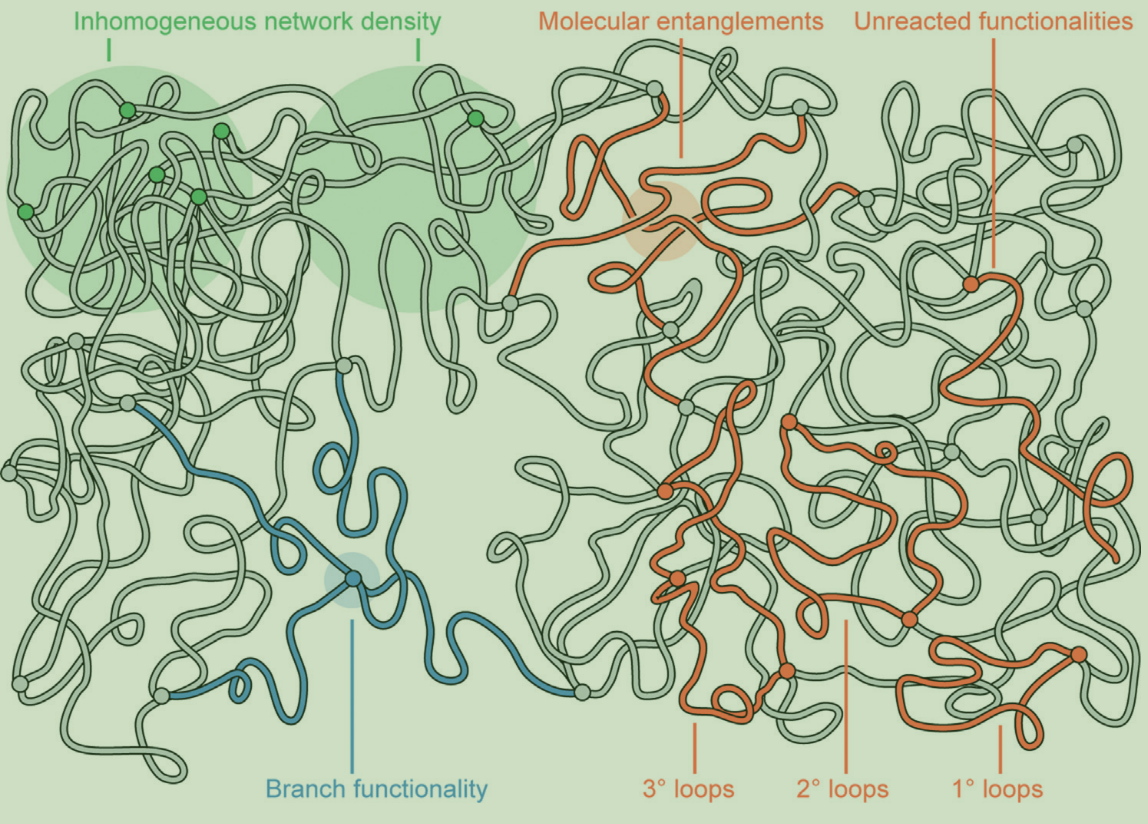
\includegraphics[width=0.8\textwidth]{figs/multilengthTopology.png}
    \caption{Multilength stuff. Scale from 10 to 100 nm shown in green, 1 to 10 nm shown in red and <1 nm shown in blue. }\label{fig:lengthScales}
\end{figure}

\subsection{Basic properties of Polymer Networks} 

\paragraph{Elasticity} The physical explanation of rubber elasticity comes from the reduction in conformational entropy that occurs as a strand in a network is stretched, this process is often modeled as the unwinding of flexible, random coils. 
Once the external stretching force is removed, an elastic entropic force restores the strands to their unstretched and higher entropy state. 
Therefore, it is concluded that network strands act as entropic molecular springs\citep{guPolymerNetworksPlastics2020}. 

\paragraph{Swelling} Polymer networks constructed from strong (e.g., covalent) bonds typically do not dissolve in solvents. 
Instead, such networks absorb solvent up to an equilibrium concentration and undergo a concomitant increase in volume. 
The equilibrium degree of swelling is dictated by a balance between the free energy of polymer-solvent mixing and the free energy cost of expanding the network, which is expressed by the Flory–Rehner equation[11,133]\footnote{for isotropic swelling of an affine polymer network [Eq. (12)]:
    \begin{gather*}
        \ln(1-\phi_{\mathrm{eq}}) + \phi_{\mathrm{eq}} + \xi\phi^2_{eq} = \eta_{eff}V_1(\phi_{\mathrm{eq}}/2-\phi^{1/3}_{eq})
    \end{gather*}
}

\paragraph{Viscoelasticity} Polymeric materials exhibit both viscous and elastic characteristics upon deformation, meaning that their properties may vary with the time scale or frequency at which measurements are performed. 
To characterize this viscoelasticity with respect to tensile, compressive, or shear deformation, several types of experimental measurements are commonly applied, such as stress relaxation, creep, and oscillatory shear tests\citep{guPolymerNetworksPlastics2020}. 

\subsection{Structure and mechanical response}




\paragraph{Covalent Adaptable Networks} Covalent adaptable networks (CANs) are produce by incroporating dynamic covalent bonds into convalent polymer networks, which alows for stimulus-induced reconfiguration of networks to reduce stresses or heal damage.
As a result, CANs not only exhibit the robust mechanical properties typical of thermosets but they can also possess the processability and relaxation behavior of thermoplastics.
Depending on the exchange mechanism, CANs may be further classified into two groups: dissociative CANs and associative CANs\citep{guPolymerNetworksPlastics2020}\footnote{A distinguishing characteristic between dissociative and associative CANs is that associative CANs display a constant crosslinking density with respect to temperature.
Since the rate of stress relaxation of these networks depends on the rate of bond rearrangement, the associative bond exchange mechanism is reflected in a viscosity with Arrhenius-like temperature dependence (Figure 9 C).
}.

\paragraph{Microporus Polymer Networks} Microporous materials are defined as materials containing interconnected pores of less than 2 nm in diameter on average. 
Due to their large surface area, many conventional microporous materials (e.g., zeolites, activated carbons) are widely used as catalysts, sorbents, and separation membranes. 





\begin{comment}
Due to their strong bonds, covalent polymer networks possess high mechanical strength across a wide range of conditions. 

While such mechanical stability enables their use in daily life, 

Many emerging applications and environmental sustainability concerns demand unconventional properties of polymernetworks, such as reprocessability, repairability upon damage, and adaptability to different environments.


Polymer networks with rapid stress relaxation that can heal when damaged (“self-healing”) are often constructed from non-covalent network bonds (e.g., metal–ligand coordination, host–guest interactions, hydrogen bonding, and hydrophobic interactions) that facilitate energy dissipation and structural reorganization. 
\end{comment}





\section{Applications}

\subsection{Rheology/stress}\label{ch1:NetworkStructure}

Main review:\citep{guPolymerNetworksPlastics2020,sheikoArchitecturalCodeRubber2019}

\paragraph{Bridge of the experiments and interpretation} Hysteresis curves to get the sotred energy and the dissipated energy.

\paragraph{Name some network structures} The correlation between the structure with the hysteresis loops

\paragraph{Link to mechanical response} Same as before.


\paragraph{What if we can change the structure on command and in real time?} Bridge to crosslinkers.

\paragraph{How crosslinking affects the mechanical response}

\begin{comment}
These include one-step procedures like polymerization and parallel cross-linking of multifunctional monomers, as well as multiple step procedures involving synthesis of polymer molecules having reactive groups and their subsequent cross-linking, possibly also by reacting polymers with suitable cross-linking agents\citep{priyaComprehensiveReviewHydrogel2024}. 

The polymer engineer can design and synthesize polymer networks with molecular-scale control over structure such as cross-linking density and with tailored properties, such as biodegradation, mechanical strength, and chemical and biological response to stimuli\citep{priyaComprehensiveReviewHydrogel2024}.

In general, the three integral parts of the hydrogels preparation are monomer, initiator, and cross-linker. 
To control the heat of polymerization and the final hydrogels properties, diluents can be used, such as water or other aqueous solutions\citep{ahmedHydrogelPreparationCharacterization2015a}. 
Then, the hydrogel mass needs to be washed to remove impurities left from the preparation process\citep{ahmedHydrogelPreparationCharacterization2015a}. 
These include nonreacted monomer, initiators, cross-linkers, and unwanted products produced via side reactions\citep{ahmedHydrogelPreparationCharacterization2015a}.

\end{comment}


Crosslinking is another essential process that can be controlled and intentionally modified using ionizing radiations\citep{priyaComprehensiveReviewHydrogel2024}. 




\begin{comment}

-------------------------------------------------

cross-linked polymer

In general, the cross-linkers increases the molecular weight of the polymer chains, which, in turn, limits their translational movement and decreases the solubility of the polymer\citep{priyaComprehensiveReviewHydrogel2024}.

Controlling the crosslinking process with ionizing radiations can be achieved by maniipulating various parameters during exposure, such as exposure time of radiaiton, frquency, temperature and pressure\citep{priyaComprehensiveReviewHydrogel2024}.




-------------------------------------------------

Hydrogels have received considerable attention in the past 50 years, due to their exceptional promise in wide range of applications [2–4]\citep{ahmedHydrogelPreparationCharacterization2015a}. 

They possess also a degree of flexibility very similar to natural tissue due to their large water content\citep{ahmedHydrogelPreparationCharacterization2015a}.

Recently, hydrogels have been defined as two- or multicomponent systems consisting of a three-dimensional network of polymer chains and water that fills the space between macromolecules\citep{ahmedHydrogelPreparationCharacterization2015a}.

Hydrogels are three-dimensional networks of hydrophilic polymers that can absorb and retain large amounts of water while maintaining their structure\footnote{Their ability to retain a large amount of water is due to their 3D structure, which gives them a gel-like appearance and behaviour.}\citep{priyaComprehensiveReviewHydrogel2024}. 

Crosslinkers play a crucial role in providing secondary interactions with biological tissues, and the presence of hydrophilic groups in the polymer chains enhances water uptake [10]\citep{priyaComprehensiveReviewHydrogel2024}. 

These methods allow researchers to create hydrogels with specific properties suitable for various applications such as tissue engineering, biomedicine, and sensing\citep{priyaComprehensiveReviewHydrogel2024}. 
The properties of hydrogels can be tailored based on the nature and arrangement of their constituent monomers, as well as the preparation method employed\citep{priyaComprehensiveReviewHydrogel2024}.


\textbf{Types of Hydrogels} or classification

From\citep{priyaComprehensiveReviewHydrogel2024} 
\begin{enumerate}
    \item Natural Polymer: 
            Natural polymer-derived hydrogels, sourced from plants or animals like polysaccharides and proteins.
            These hydrogels are adept at absorbing and retaining water, effectively managing pesticide release in soil to boost efficacy and minimize environmental harm caused by excessive application.
            Despite challenges like mechanical strength variations inherent in natural sources, natural polymer-derived hydrogels hold great promise for sustainable agriculture and environmental conservation.
            Examples: Cellulose, derivatives such as crboxymethyl celluose, Chitosan, Sodium alginate
    \item Synthetic Polymer: 
            Synthetic polymer hydrogels, such as those made from polyacrylamide (PAM) and PVA.
            controllable structures, mechanical strength, and chemical stability.
            PAM is especially favoured for its water retention and non-toxic nature, making it prevalent in biomedicines and agriculture. 
            However, the use of PAM comes with concerns. 
            Acrylamide, used in PAM synthesis, is potentially neurotoxic and may release unreacted particles, posing environmental and health risks. 
            Additionally, these hydrogels have low biodegradability, causing environmental residues and potential contamination. 
            Production of these synthetic polymers often involves harmful chemicals, increasing costs and raising further health and environmental concerns
    \item Natural-Synthetic Polymer: 
            blending natural polymers like alginate and xanthan gum with synthetic counterparts such as PAM and PVA.
            These hydrogels enhance biodegradability and biocompatibility, mitigate long-term soil and water contamination risks, and provide robust mechanical strength and chemical stability.
\end{enumerate}



\end{comment}
 



\newpage
      % Chapter 1 Intro



%======================================================================
\chapter{Theoretical framework}\label{ch2:Problem}

\markright{State of the Art}
%======================================================================

\section{Soft colloids}\label{ch2:SoftColloids}

\paragraph{Argument} Why we can use a simulation protocol for microgels to modeled hydrogels?

\begin{itemize}
    \item Why we can model hydrogels as Soft colloids?
    \item Idea of patchy particles and insterpretaion of interaction rules
    \item teaser of simulation experiments
\end{itemize}


Hydrophilic gels that are usually referred to as hydrogels are networks of polymer chains that are sometimes found as colloidal gels in which water is the dispersion medium [1]\citep{ahmedHydrogelPreparationCharacterization2015a}.


\section{Molecular dynamics}\label{ch2:MD}

\begin{itemize}
    \item Langevin equation
    \item Velocity Verlet
\end{itemize}

\subsection{Langevin dynamics}

From a general point of view there are two types of methods to make a quatitative description of systems: one focused on simulating dynamics at the microscale, and the other dedicated to deriving or establishing evolutionary equations at the macroscale\citep{wangMultiscaleModelingSimulation2025}.
Since we assume that the a microgel's mechanical response derives from its internal structure\footnote{Poner citas que desmuestrén que no es hipótesis, si no que se sabe} we choose to simulate the dynamics at the microscale.
Additionally, by treating the microgel as a colloid, permits applying Brownian motion theory to model its response under shear deformation. 
Finally, there are two commonly used mathematical frameworks to model the Brownian motion, the continuous time random walk (CTRW) model and the Langevin equation\citep{wangMultiscaleModelingSimulation2025}, in this work we decided\footnote{Supongo que eventualmente justificaré la desición.} to use the langevin dynamics mathematical framework.

This is because, the solid phase of the colloid has a large mass and will change their momenta after many collisions with the solvent molecules and the picture which emerges is that of the heavy particles forming a system with a much longer time scale than the solvent molecules\citep{Thijssen2007} and Langevin theory takes advantage of this difference in time scale to eliminate the details of the degrees of freedom of the solvent particles and represent their effect by stochastic and dissipative forces allowing longer simulations that would be impossible if the solvent were explicitly included\citep{pastorTechniquesApplicationsLangevin1994}.
However, the representation of the solvent by a stochastic and dissipative force, introduce the problem of characterize two very different timescales, one associated with the slow relaxation of the initial velocity of the brownian particle and another linked to the frequent collisions that the brownian particle suffers with particles of the bath\citep{tsl2006}\footnote{Para traer a colación la sensibilidad de la respuesta mecánica al parámetro de damp.}. 
Therefore, two terms are used to create a mathematical representation of the solvent: a frictional force proportional to the velocity of the brownian particle and a fluctuating force. 
Hence,
\begin{gather}
    m\dv{\vec{v}(t)}{t}=\vec{F}(t)-m\gamma\vec{v}(t)+\vec{R}(t).\label{eqn:BrownianDyn1}
\end{gather}
The friction constant $\gamma$\footnote{Cuidado con las unidades. Hacer análisis dimensional, porque por la condición de correlación en $R$, $\gamma$ ocupa tener unidades de masa entre tiempo, pero en la ecuación, solo ocupa unidades de $1/s$.} parametrises the effect of solvent damping and activation and is commonly referred to as the collision frequency in the simulation literature, even though formally a Langevin description implies that the solute suffers an infinite number of collisions with infInitesimally small momentum transfer.
Also, the fact that the second term is not a function of the position of any of the particles involves the neglect of involves the neglect of hydrodynamic interaction or spatial correlation in the friction kernel spatial correlation in the friction kernel\citep{pastorTechniquesApplicationsLangevin1994}.
On the other hand, $\vec{R}(t)$\footnote{No me acuerdo en donde está que se puede asumir que tiene distribución gaussiana.} is a ``random force''subject to the following conditions
\begin{align*}
    \expval{\vec{R}(t)} &= 0 \\
    \expval{\vec{R}(t)\vec{R}(t')} &= 2k_{B}T\gamma\delta\qty(t-t') 
\end{align*}
The no time correlation is equivalent to assuming that the viscoelastic relaxation of the solvent is very rapid with respect to solute motions\footnote{Grote land Hynes [26] have investigated this assumption for motions involving barrier crossing and have found that while it is seriously in error for passage over sharp barriers (such as 12 recombination); it is quite adequate for conformational transitions such as might be found in polymer motions.\citep{pastorTechniquesApplicationsLangevin1994}}.

In comparing the results of Langevin dynamics with those of other stochastic methods [28-31], the relevant variable is the velocity relaxation time, $\tau_{v}$ which equals $\gamma^{-1}$\citep{pastorTechniquesApplicationsLangevin1994}
The Langevin equation improves conformational sampling over standard molecular dynamics\citep{paquetMolecularDynamicsMonte2015}.

\begin{itemize}
    \item Hablar acerca de que la fuerza aleatoria puede tener distribución gaussiana, pero no necesariamente.
    \item hablar de la ecuación de Green-Kubo: \[\eta=\frac{V}{k_B T}\int_{0}^{\infty}\expval{\sigma_{xy}(t)\sigma_{xy}(0)}\mathrm{d}t\]
    \item No se que tanto hablar de la idea de correlación y su aplicación en estos temas.
\end{itemize}

\subsection{Velocity Verlet}

\paragraph{Overview of the method}

\paragraph{Characteristics of the method}


\section{Mechanical response}\label{ch2:MechResponse}

\begin{itemize}
    \item Macroscopic Stress (Cauchy)
    \item Microscopic Stress (PhD Thesis of pointwise fields )
\end{itemize}

\subsection{Stress}

\paragraph{Introductory paragraph} To characterize the behaviour of materials, constitutive relations serve as an input to the continuum theory\dots\footnote{Capaz e ir introduciendo ideas del Clausius\citep{clausiusXVIMechanicalTheorem1870}}

This derivation can be found in the apendix of\citep{admalUnifiedInterpretationStress2010}\footnote{Describe more if what is done in this article}.\footnote{(Eventualmente pondré esto en párrafo) Notation:
    $\bm{\sigma}$ Tensor, $\vec{\sigma}$ vector, $\sigma_{i,j}$ tensor, $\overline{\sigma}$ time average, 
}
Consider a system of $N$ interacting particles with each particle position given by
\begin{equation}
    \vec{r}_{\alpha} = \vec{r} + \vec{s}_{\alpha}\label{eqn:DerVirTen1},
\end{equation}
where $\vec{r}$ is the position of the center of mass of the system and $\vec{s}_\alpha$ is the position of each point relative to the center of mass.
Hence, we can express the momentum of each particle as
\begin{equation}
    \vec{p}_\alpha = m_\alpha\qty(\dot{\vec{r}}+\dot{\vec{s}}_\alpha) = m_\alpha\qty(\dot{\vec{r}}+\vec{\upsilon}_\alpha^{\mathrm{rel}}).\label{eqn:DerVirTen2}
\end{equation}
Before starting the procedure, lets take into account that the center of mass of the system is given by
\begin{equation}
    \vec{r} = \frac{\sum_{\alpha}m_\alpha\vec{s}_\alpha}{\sum_{\alpha}m_\alpha}\label{eqn:DerVirTen3},
\end{equation}
and by replacing~\eqref{eqn:DerVirTen1} in~\eqref{eqn:DerVirTen2} we get the following relations, which will be used later,
\begin{equation}
    \sum_\alpha m_\alpha\vec{r}_\alpha = \vec{0},\quad
    \sum_\alpha m_\alpha\vec{\upsilon}_\alpha^{\mathrm{rel}} = \vec{0}.\label{eqn:DerVirTen4}
\end{equation}

Now we can start by computing the time derivative of tensorial product $\vec{r}_\alpha\otimes\vec{p}_\alpha$\footnote{It is interesting to note that the tensorial product $\vec{r}_\alpha\otimes\vec{p}_\alpha$ has units of action and by tacking the time derivative we are dealing with terms that has units of energy.
},
\begin{equation}
    \dv{t}\qty(\vec{r}_\alpha\otimes\vec{p}_\alpha) = 
    \underbrace{\vec{\upsilon}_\alpha^{\mathrm{rel}}\otimes\vec{p}_\alpha}_{\mathrm{Kinetic~term}} 
        +
        \underbrace{\vec{r}_\alpha\otimes\vec{f}_\alpha}_{\mathrm{Virial~term}},\label{eqn:DerVirTen5}
\end{equation}
which is known as the \textit{dynamical tensor virial theorem} and it is simply an alternative form to express the balance of linear momentum.
This theorem becomes useful after making the assumption that there existis a time scale $\tau$, which is short relative to macroscopic processes but long relative to the characteristic time of the particles in the system, over which the particles remain close to their original positions with bounded positions and velocities.
Taking advantage of this property we can compute the time average of~\eqref{eqn:DerVirTen5},
\begin{equation}
    \frac{1}{\tau}\qty(\vec{r}_\alpha\otimes\vec{p}_\alpha)\bigg|_{0}^{\tau} = 
    \overline{\vec{\upsilon}_\alpha^{\mathrm{rel}}\otimes\vec{p}_\alpha} 
        +
    \overline{\vec{r}_\alpha\otimes\vec{f}_\alpha}.\label{eqn:DerVirTen6}
\end{equation}
Assuming that $\vec{r}_\alpha\otimes\vec{p}_\alpha$ is bounded, and the time scales between microscopic and continuum processes are large enough, the term on the left-hand side can be as small as desired by tacking $\tau$ sufficiently large and by summing over all particles we achieve the \textit{tensor virial theorem}:
\begin{equation}
    \overline{\bold{W}} = -2\overline{\bold{T}},\label{eqn:DerVirTen7}
\end{equation}
where
\begin{equation}
    \overline{\bold{W}} = \sum_\alpha\overline{\vec{r}_\alpha\otimes\vec{f}_\alpha}\label{eqn:DerVirTen8}
\end{equation}
is the time-average virial tensor and
\begin{equation}
    \overline{\bold{T}}=\frac{1}{2}\sum_\alpha\overline{\vec{\upsilon}_\alpha^{\mathrm{rel}}\otimes\vec{p}_\alpha}\label{eqn:DerVirTen9}
\end{equation}
is the time-average kinetic tensor.
This expression for the tensor virial theorem applies equally to continuum systems that are not in macroscopic equilibrium as well as those that are at rest.

The assumption of the difference between the time scales allow us to simplify the relation by replacing~\eqref{eqn:DerVirTen2} in~\eqref{eqn:DerVirTen9}, so that,
\begin{equation}
    \overline{\bold{T}}=
        \frac{1}{2}\sum_\alpha m_\alpha\overline{\vec{\upsilon}_\alpha^{\mathrm{rel}}\otimes\vec{v}_\alpha^{\mathrm{rel}}}
        +
        \frac{1}{2} \left[\overline{\sum_\alpha m_\alpha\vec{\upsilon}_\alpha^{\mathrm{rel}}}\right]\otimes\dot{\vec{r}}\label{eqn:DerVirTen10},
\end{equation}
which is not the simplification we expected, however, by the relations from~\eqref{eqn:DerVirTen4}, equation~\eqref{eqn:DerVirTen10} simplifies to\footnote{No estoy muy seguro si incluir una discusión acerca del término cinético en la expresión del virial. Posiblemente un párrafo\dots posiblemente lo ponga en la interpretación del teorema.
También, no se si ir metiendo interpretación durante la derivación o no, pero bueno.}
\begin{equation}
    \overline{\bold{T}}=
        \frac{1}{2}\sum_\alpha m_\alpha\overline{\vec{\upsilon}_\alpha^{\mathrm{rel}}\otimes\vec{\upsilon}_\alpha^{\mathrm{rel}}}\label{eqn:DerVirTen11}.
\end{equation}
On the other hand, instead of reducing the expression, we start to create the conection with the Cauchy stress tensor by distributing~\eqref{eqn:DerVirTen8} into an internal and external contributions,
\begin{equation}
    \overline{\bold{W}} = 
    \underbrace{\sum_\alpha\overline{\vec{r}_\alpha\otimes\vec{f}_\alpha^{\mathrm{int}}}}_{\overline{\bold{W}}_{\mathrm{int}}}
        +
        \underbrace{\sum_\alpha\overline{\vec{r}_\alpha\otimes\vec{f}_\alpha^{\mathrm{ext}}}}_{\overline{\bold{W}}_{\mathrm{ext}}}.\label{eqn:DerVirTen12}
\end{equation}
The time-average internal virial tensor takes into account the interaction between particle $\alpha$ with the other particles in the system, meanwhile, the time-average external virial tensor considers the interaction with atoms outside the system, via a traction vector $\vec{t}$ and external fields acting on the system represented by $\rho\vec{b}$, where $\rho$ is the mass density of it and $\vec{b}$ is the body force per unit mass applied by the external field.
Therefore we can express the following,
\begin{equation}
    \sum_\alpha\overline{\vec{r}_\alpha\otimes\vec{f}_\alpha^{\mathrm{ext}}}
    :=
    \int_{\delta\Omega}\vec{\xi}\otimes\vec{t}dA 
    +
    \int_{\Omega}\vec{\xi}\otimes\rho\vec{b}dV.\label{eqn:DerVirTen13}
\end{equation}
Where $\vec{\xi}$ is a position vector within the domain $\Omega$ occupied by the system of particles with a continuous closed surface $\delta\Omega$.
Assuming that $\Omega$ is large enough to express the external forces acting on it in the form of the continuum traction vector $\vec{t}$.

With this we can substitute the traction vector with $\vec{t}=\bm{\sigma}\vec{n}$, where $\bm{\sigma}$ represent the Cauchy stress tensor and applying the divergence theorem in~\eqref{eqn:DerVirTen13}, we have 
\begin{equation}
    \overline{\bold{W}}_{\mathrm{ext}}
     =\int_{\Omega}
        \left[
            \vec{\xi}\otimes\rho\vec{b}+\mathrm{div}_{\vec{\xi}}\qty(\vec{\xi}\otimes\bm{\sigma})
        \right]dV
        =
    \int_{\Omega}
        \left[
            \bm{\sigma}^{\mathrm{T}}
            +
            \vec{\xi}\otimes\qty(\mathrm{div}_{\vec{\xi}}\bm{\sigma}+\rho\vec{b})
        \right]dV\label{eqn:DerVirTen14}
\end{equation}
Since we assume that we are under equilibrium conditions, the term $\mathrm{div}_{\vec{\xi}}\bm{\sigma}+\rho\vec{b}$ is zero~\eqref{eqn:DerVirTen14} it simplifies to
\begin{equation}
    \overline{\bold{W}}_{\mathrm{ext}}
    =V\bm{\sigma}^{\mathrm{T}}\label{eqn:DerVirTen15}.
\end{equation}
By tacking into account that we integrate over the domain $\Omega$ we can say that we compute the spatial average of the Cauchy stress tensor,
\begin{equation}
    \bm{\sigma}_{\mathrm{av}} =\frac{1}{V}\int_\Omega\bm{\sigma}dV\label{eqn:DerVirTen16},
\end{equation}
in which $V$ is the volume of the domain $\Omega$.
Replacing~\eqref{eqn:DerVirTen15} into~\eqref{eqn:DerVirTen12}, the tensor virial theorem~\eqref{eqn:DerVirTen7} can be expressed as,
\begin{equation}
    \sum_\alpha\overline{\vec{r}_\alpha\otimes\vec{f}_\alpha^{\mathrm{int}}}
    +
    V\bm{\sigma}_{\mathrm{av}}^{\mathrm{T}}
    =
    -\sum_\alpha m_\alpha\overline{\vec{\upsilon}_\alpha^{\mathrm{rel}}\otimes\vec{\upsilon}_\alpha^{\mathrm{rel}}}.\label{eqn:DerVirTen17}
\end{equation}
Finally, solving for the Cauchy Stress tensor we get,
\begin{equation}
    \bm{\sigma}_{\mathrm{av}}
    =
    -\frac{1}{V}
    \left[
        \sum_\alpha\overline{\vec{f}_\alpha^{\mathrm{int}}\otimes\vec{r}_\alpha}
        +
        \sum_\alpha m_\alpha\overline{\vec{\upsilon}_\alpha^{\mathrm{rel}}\otimes\vec{\upsilon}_\alpha^{\mathrm{rel}}}
    \right],\label{eqn:DerVirTen18}
\end{equation}
an expression that describe the macroscopic stress tensor in terms of microscopic variables\footnote{It is important to acknowledge that several mathematical subtleties were not taken into consideration, however all the mathematical formality is adressed by Nikhil Chandra Admal and E. B. Tadmor in~\citep{admalUnifiedInterpretationStress2010}}.

To end the section it is important to show that~\eqref{eqn:DerVirTen18} is symmetric.
Therefore, we rewrite the internal force as the sum of forces between the particles,
\begin{equation}
    \vec{f}^{\mathrm{int}}_\alpha = \sum_{{\beta}_{\beta\neq\alpha}}\vec{f}_{\alpha\beta}\label{eqn:DerVirTen19},
\end{equation}
and substituting~\eqref{eqn:DerVirTen19} into~\eqref{eqn:DerVirTen18}, we have
\begin{equation}
    \bm{\sigma}_{\mathrm{av}}
    =
    -\frac{1}{V}
    \left[
        \sum_{{\alpha,\beta}_{\beta\neq\alpha}}\overline{\vec{f}_{\alpha\beta}\otimes\vec{r}_\alpha}
        +
        \sum_\alpha m_\alpha\overline{\vec{\upsilon}_\alpha^{\mathrm{rel}}\otimes\vec{\upsilon}_\alpha^{\mathrm{rel}}}
    \right].\label{eqn:DerVirTen20}
\end{equation}
Due to the property $\vec{f}_{\alpha\beta}=-\vec{f}_{\beta\alpha}$ we obtain the following identity
\begin{equation}
    \sum_{{\alpha,\beta}_{\beta\neq\alpha}}\vec{f}_{\alpha\beta}\otimes\vec{r}_\alpha 
    =
    \frac{1}{2}\sum_{{\alpha,\beta}_{\beta\neq\alpha}}\left(\vec{f}_{\alpha\beta}\otimes\vec{r}_\alpha+\vec{f}_{\beta\alpha}\otimes\vec{r}_\beta\right)
    =
    \frac{1}{2}\sum_{{\alpha,\beta}_{\beta\neq\alpha}}\vec{f}_{\alpha\beta}\otimes\left(\vec{r}_\alpha-\vec{r}_\beta\right).\label{eqn:DerVirTen21}
\end{equation}
Therefore, by replacing the identity of~\eqref{eqn:DerVirTen21} into~\eqref{eqn:DerVirTen20}, we have
\begin{equation}
    \bm{\sigma}_{\mathrm{av}}
    =
    -\frac{1}{V}
    \left[
        \frac{1}{2}
        \sum_{{\alpha,\beta}_{\beta\neq\alpha}}\overline{\vec{f}_{\alpha\beta}\otimes\left(\vec{r}_\alpha-\vec{r}_\beta\right)}
        +
        \sum_\alpha m_\alpha\overline{\vec{\upsilon}_\alpha^{\mathrm{rel}}\otimes\vec{\upsilon}_\alpha^{\mathrm{rel}}}
    \right],\label{eqn:DerVirTen22}
\end{equation}
expressed with indexical notation and using the eistein summation convention,
\begin{equation}
    \sigma^{\mathrm{av}}_{ij}
    =
    -\frac{1}{V}
    \left[
        \frac{1}{2}
        \sum_{{\alpha,\beta}_{\beta\neq\alpha}}\overline{f^{\alpha\beta}_{i}r^\alpha_{j} + f^{\beta\alpha}_{i}r^\beta_{j}}
        +
        \sum_\alpha m_\alpha\overline{\upsilon^{\alpha~\mathrm{rel}}_{i}\upsilon^{\alpha{\mathrm{rel}}}_j}
    \right],\label{eqn:DerVirTen23}
\end{equation}
which is the same expression implemented in~LAMMPS\citep{LAMMPS}.\footnote{No se si poner la referencia a la pagina de documentacion\href{https://docs.lammps.org/compute_stress_atom.html}{https://docs.lammps.org/compute\_stress\_atom.html}}


\newpage
      % Chapter 2 Theoretical framework
\chapter{Patchy particle scheme for hydrophilic polymeric networks}

Now that we have covered the theoretical framework, we can delve into the numerical tools that will help us find relations between the polymeric network and the mechanical response.
First, we will describe the patchy particle scheme for simulating PNIPAM cross-linked networks.
Then, we will describe the numerical simulation protocol.
Next, we will introduce the LAMMPS package and explain how it can be used to simulate these systems.
Finally, we will present and analyze the simulation results.

\section{Simulation protocol}

One of the microgels that has been the focus of significant research is the type that is based on PNIPAM cross-linked networks.
In the article \textit{In silico Synthesis of Microgel Particles}\citep{gnanSilicoSynthesisMicrogel2017}, the authors present a flexible numerical protocol capable of designing individual microgel particles based on PNIPAM corr-linked networks. 
This protocol can generate particles with properties comparable to the experimental ones.
In this project, we employ a similar protocol to explore its versatility and identify a numerical tool that can facilitate connections between network configuration and mechanical response.

Our primary focus is on creating networks without spherical confinement and without mimicking the swelling behavior of PINIPAM microgels with temperature.
Therefore, the central strategy involves the implementation of a binary mixture of patchy particles to generate a disorded polymeric network structure, followed by the application of shear deformation.
The primary benefit of this protocol is that previous numerical efforts in microgel modeling have predominantly concentrated on unrealistic networks consisting of chains of equivalent length, frequently establishing cross-linked connections on crystalline lattice regions or where closed polymer networks are assembled by directly integrating randomly dispersed cross-linkers with polymer chains.

\subsection{Patchy particles representation}

A patchy particle\citep{bianchiPhaseDiagramPatchy2006,bianchiTheoreticalNumericalStudy2008} can be defined as a sphere with radius $r$ containing $n$ spheres of radius $l<r$ on its surface.
The smaller spheres are typically referred to as ``patches'' and the number of patches is often refer to as ``functionality''.
The center of the patches can be placed on the surface of the central particle. 
However, it can also be modified to be at a point inside the enclosed volume of the main particle.

The implementation of patchy particles as monomers and crosslinkers is a highly effective strategy.
This is due to the fact that it facilitates the integration of the infinitesimal representation by the Langevin dynamics with a particle that possesses volume and functionality.
The functionality representation is important because it allows for the representation of the monomer and cross-linker molecules that can form a polymeric network.
However, it is important to recognize that the geometry of the monomers and functional groups is assume to be spherical.

Finally, to define the volume of the particle, a repulsive pairwise interaction is defined between the central particles.
Meanwhile, to the formation of a polymeric network is facilitated by an attractive pairwise interaction defined between patches.
Because this model is designed to simulate the final network, not the synthesis process, the pairswise interaction between central particles and patches is not defined.

In contrast, the softness explain by particle interactions is characterized by the form of the repulsive pair potential between two particles.
Finally, the particle volume fraction contributes to the ability of the particles to deform or compress, in contrast to hard spheres\footnote{The patchy particles are hard spheres, but the hydrogel network is a soft ``particle''}\citep{vlassopoulosTunableRheologyDense2014}.

\subsection{Description of the system}

\paragraph{Interaction potentials} We start by describing the interaction potentials between patchy particles.
The interaction between the central particles is modeled with a Weeks-Chandler-Andersen repulsive potential,
\begin{gather}
    U_{WCA}(r_{i,j}) =\left\{ 
        \begin{array}{ll}
            4\epsilon_{i,j}\left[\qty(\frac{\sigma}{r_{i,j}})^{12}-\qty(\frac{\sigma}{r_{i,j}})^6\right]+\epsilon_{i,j}, & r_{i,j}\in[0,2^{1/6}\sigma], \\
            0, & r_{i,j}>2^{1/6}\sigma
        \end{array}
\right.
    ,\label{eqn:CL-MO_interaction}
\end{gather}
where $r_{i,j}$ is the distance between the center of the central particles, $\sigma$ is the diameter of the particles and $\epsilon_{i,j}$ is the energy of the interacton.
On the other hand, the patch-patch interaction is modeled with an attractive potential,
\begin{gather}
    U_{\mathrm{patchy}}\qty(r_{\mu\upsilon}) = \left\{
        \begin{array}{ll}
            2\epsilon_{\mu\upsilon}\left(\frac{\sigma_p^4}{2 r_{\mu\upsilon}^4}-1\right)\exp\left[\frac{\sigma_p}{\qty(r_{\mu\upsilon}-r_{c})}+2\right], & r_{\mu\upsilon}\in\qty[0,r_c], \\
            0, & r_{\mu,\upsilon}>r_c,
        \end{array}
            \right.\label{eqn:patch-patch_interaction}
\end{gather}
where $r_{\mu\upsilon}$ is the distance between two patches, $\sigma_p$ is the diameter of the patches, $r_c$ is the cut distance of interaction set to $1.5\sigma_p$ and $\epsilon_{\mu,\upsilon}$ is the interaction energy between the patches.
This potential can be interpreted as a reversible interaction.

\begin{figure}[ht!]
    \centering
    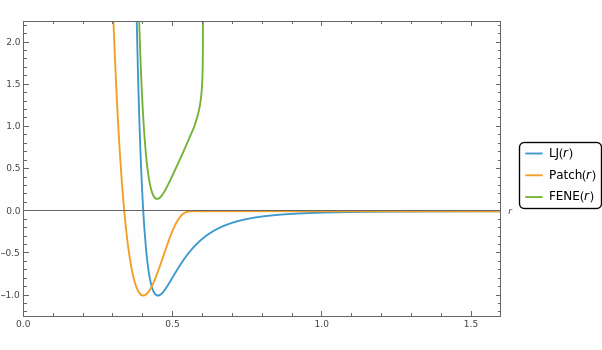
\includegraphics[width=0.8\textwidth]{figs/numerical/patchpatch.png}
    \caption{Comparisson of attractive interaction potentials}\label{fig:patchpatchpot}
\end{figure}

It is important to say that if we let the polymeric network form with only those potentials, the patches are going to form cluster of more than 2 patches, which is not desirable, because it does not follows the single bond per patch condition.
Hence, the interaction between patches is complemented by a three-body repulsive potential, defined in terms of~\eqref{eqn:patch-patch_interaction}, that provides an efficient bond-swapping mechanism making possible to easily equilibrate the system at extremely low temperatures, while at the same time, reataining the single bond per patch condition\citep{sciortinoThreebodyPotentialSimulating2017},
\begin{gather}
    U_{\mathrm{swap}}(r_{l,m},r_{l,n}) = w\sum_{l,m,n}\epsilon_{m,n}U_3\qty(r_{l,m})U_3\qty(r_{l,n}),\quad r_{l,n}\in\qty[0,r_c],\label{eqn:swap_interaction}
\end{gather}
where
\begin{gather}
    U_{3}\qty(r) = \left\{
        \begin{array}{ll}
            1 & r\in\qty[0,r_{\min}], \\
            -U_{\mathrm{patchy}}\qty(r)/\epsilon_{m,n}, & r\in\qty[r_{\min},r_c]
        \end{array}
        \right.\label{eqn:swapmod_interaction}.
\end{gather}
The sum in~\eqref{eqn:swap_interaction} runs over all triples of bonded patches (patch $l$ bonded both with $m$ and $n$).
$r_{l,m}$ and $r_{l,n}$ are the distances between the reference patch and the other two patches.
The parameter $\epsilon_{m,n}$ is the energy of repulsion and $w$ is used to tuned the swapping ($w=1$) and non-swapping bonds ($w\gg1$). 
The cut off distance $r_c$ is the same as in the potential of interaction between patches, meanwhile the minimum distance $r_{\min}$ is the distance at the minimum of~\eqref{eqn:patch-patch_interaction}, \textit{i.e.} $\epsilon_{m,n}\equiv\abs{U_{\mathrm{patchy}}(r_{\min})}$.
Finally, the energy of interaction between crosslinker patches ($\epsilon_{\mu^i,\mu^i}$) are set to $0$ to allow only crosslinker-monomer and monomer-monomer bonding (figure~\ref{fig:intento2}).

\paragraph{Polymeric network parameters}
Now that the interaction between pathcy particles have been described, we can describe the control parameters for the simulations.
We set a constant number of patchy particles $N_p$, a packing fraction $\phi$ and a cross-link concentration $c$. 
From this parameters we compute the volume of the box and the number of patchy particles of functionality 2 (PB) and the patchy particles of functionality 4 (PA).

Due to limitations related to time and computing resources, we have set the total number of particles to be $N_p=\num{8000}$.
This is a lower number of particles when compared with other simulations[cites].
Therefore, in order to compensate, we take the mean of five experiments.
This is equivalent to simulating a system of \num{40000} particles, but with a more manageable computational requirements.

Once we set the parameters for the synthesis, the volume of the box was calculated by determining the volume of the patchy particles A and B, and then scaling those values by the number of particles and the desired packing fraction.
\begin{align*}
    V_{\mathrm{box}} &= \frac{N_{\mathrm{patchyA}}V_{\mathrm{patchyA}}+N_{\mathrm{patchyB}}V_{\mathrm{patchyB}}}{\phi}
\end{align*}
The number of patchy particle of type A is computed as $N_{\mathrm{patchyA}} = c N_p$ and the number of patchy particles of type B as $N_{\mathrm{patchyB}}= N_p - N_{\mathrm{patchyA}}= N_p(1 - c )$.
Finally, the temperature was set to be constant thru all the assembly process $T=0.05$ in Lennard-Jones units, meanwhile, the damp parameter was set to $\mathrm{damp}=0.1$.
It is important to notice that the damp controlls the viscous response from the interaction between the thermal bath and the particles, which represents the interaction between water molecules and the polymer network.

\paragraph{Deformation protocol} 
Once the synthesis of the hydrogel was set, we peform a shear deformation to the resulting polymeric network.
We select the shear deformation because shear forces dominate biological environments where hydrogels are typically deployed. 
Also, shear testing provides a more uniform stress field throughout the hydrogel sample compared to tensile testing. 
In rheological measurements using parallel plate or cone-and-plate geometries, the applied shear stress is distributed evenly across the sample, eliminating edge effects and stress concentrations that plague tensile testing.
Furthermore, shear rheometry excels at characterizing the complex viscoelastic properties that define hydrogel functionality.
Many hydrogels exhibit shear-thinning behavior that is critical for applications like injection and 3D bioprinting. 

Since we are exploring this computational methodology to characterized the mechanical response, we choose to have a constant shear rate to deform beyond the plastic deformation limit.
Also we vary the shear rate of the deformation to see the viscoelastic response of the material.
The temperature was held constant to a value of $0.05$ Lennar-Jones units and a damp on \num{0.1}.


\subsection{LAMMPS implementation}

\paragraph{Three-body potential}
%An importante technica issue to address is the tabulation of the threebody potential to introduce the swap potential into LAMMPS.
This is because the forces on all three particles $I$, $J$, and $K$ of a triplet of this type of three-body interaction potential lie within the plane defined by the three inter-particle distance vectors $\vec{r}_{IJ}$, $\vec{r}_{IK}$ and $\vec{r}_{JK}$.
This property is used to project the forces onto the inter-particle distance vectors.
Hence, we need to create a table taking that into consideration, for that we \textbf{\ldots}

Deformation.

\paragraph{fix deform} To explain how the deformation is perform.

\paragraph{fix stress} to explain how the stress tensor is computed.

\section{Results}

\subsection{Mechanical response}

Strain stress graph

\begin{figure}[ht!]
    \centering
    \includegraphics[width=\textwidth]{figs/ComputaitonalResults/strain-vs-stressxy.png}
    \caption{results from computational results test}
\end{figure}


\subsection{Network analysis}

I guess that figures of the final network and parameter of order or size of porous or whatever.

      % Chapter 3 Numerical Experiments
\chapter{Conclusion}

We conclude that we have a conclusion in two years.

The patchy particle protocol is a vlid methodology to simulate the mechanical response of polymeric networks.

In order to simulate hydrogels we need no add a FENE potential.

The reverible interactions are more sutiable to model microgel particle response.


      % Chapter 4 Conclusion

\bibliography{biblio}     % names file phdrefs.bib as my bibliography file



\end{document}
